\section{Background and Related Work}
\label{sec:background}

\subsection{Grounding}
Symbols of a symbolic system such as words in a natural language are typically processed and manipulated in a purely formal manner, without direct reference to their real-world concepts.
The question arises, how these symbols can acquire meaning and be connected to the real world without any external interpreter, in other words how the symbols can be grounded in the real world.
This is known as the symbol grounding problem \citep{Harnad1990}.
Hereby, \citet{Harnad1990} describes that a high-order \emph{symbolic representation} needs to be grounded bottom-up in two non-symbolic representations.
\emph{Iconic representations} refer to analogue representations of sensory input like for instance vision in the retina.
These representations are mapped to \emph{categorical representations} which are filtered clusters of the iconic representation.
These categories are assigned so-called elementary symbols, in which symbolic representation are grounded.

In computational models this problem is tried to be solved in multiple ways.
Recent large language models (LLMs) such as BERT \citep{Devlin2019} or GPT-3 \citep{Brown2020} are often trained on big amounts of text corpora produce impressive results on many tasks in Natural Language Processing.
Meaning of symbols emerges through relating it to its surrounding context of other symbols it appears in.
In this way, their only way of learning, how to generate language as well as solve these tasks is to find patterns of how words and sentences are used in these large corpora.
This approach is however criticized by many researchers, since the meaning of symbols is still not connected to the real world and only relies on other symbols in an infinite recursion.

In \citep{Bender2020}, the authors argue that meaning is bound to a communicative intent.
These are the purposes of why humans are using language.
The intent is always embedded in a broader context that exists outside the language itself.
This context includes the real world, but also the background knowledge of the speaker as well as interlocutors or reason for what the speaker is saying.
By grounding the intent in this context, it becomes meaningful.
Only with this step, the intent can be interpreted by the listeners.
% This intent is connected to the real world that exists outside of language, in other words it is grounded in the world.
% SD: Not just real world, also to background knowledge and what the person wants to do. 
% SD: Grounding is more related to interpretability of expressions rather than intent. Without grounding they cannot be interpreted. The intent shapes WHAT referring expressions are generated in what contexts of the real world.   Hence, intent is a meta thing connecting world, language, knowledge and agent’s experience.
% DK: first part included, referring expressions are included below (done)
This grounding is missing when models only train on abstract textual representations of the world \citep{Regier1996,Landau1998}.

\citet{Bisk2020} argues that a multimodal approach, including for instance perception as well as social context, is needed to learn meaning in a broader context.
One added modality to ground language is often visual input.
Hereby, the model needs to learn how to associate linguistic concepts in text corpora with features, extracted from visual input.
For instance, a model can learn to associate the noun "dog" with an animal seen in an image or associate the action of "jumping over" with the animal being above an object.
\cite{Roy2002} for example studies how an artificial agent can ground spatial relations with a visual scene of geometric shapes.
Hereby, the agent builds up hierarchical knowledge that is used to produce correct description in a rule-based manner.
In more recent research, complete natural language utterances as well as the visual representations are mapped into an embedding space.
By aligning both representations, natural language can be connected to a second modality.
Other research explores how to ground smaller parts of the utterances, as phrases and words and combine them compositional \citep{Larsson2018,Kollar2010}.
This might allow artificial machines to learn grounded concepts more general.

Furthermore, artificial agents can learn to ground language through dialogue, either with human tutors or with other artificial agents.
\citet{Skocaj2011} for example teach a robot different objects and concepts.
By asking questions and participating in the dialogue with a human tutor, the robot builds up and verifies beliefs, and connects them to language and its visual input.
\citet{Lauria2001} follow a similar approach where a robot is taught to follow instructions to generate a map of its physical surroundings.
By incorporating dialogue and deep-level reasoning questions the learning gains are enhanced.
How artificial agents can ground language in dialogue between each other will be studied in this thesis.
Section \ref{sec:background:language-games} gives an insight in the state of the research.


\subsection{Referring expressions}
\label{sec:background:re}
A specific case of grounding linguistic information in visual input are referring expressions.
While a general linguistic expression can be grounded in multiple regions of a visual scene, referring expressions are expected to refer to a unique region \citep{Sanchez2022}.
Given for example a visual scene with multiple pens lying on a table, the word 'pen' can be grounded in all visible objects.
A referring expression like 'the red pen on the left' in contrast would only refer to one specific object.
Referring expressions are however not limited to refer to one single entity, but might also refer to a group of objects as for instance with 'the green pens'.
Still they refer to a specific subset of entities and concepts.

Hereby, \citet{Krahmer2012} classify referring expressions into four categories:
\emph{One-place predicates} refer to one single entity in the visual scene without.
By this, the entity is identifiable without using another entity as basis.
Often, the referring expressions includes intrinsic attributes of an object or absolute locations in the scene as in 'the red pen on the left'.
\emph{Relational} referring expressions refer to entities via other entities in the scene.
Accordingly, a relating between the target entity and distractors is described.
This includes for example spatial relations like 'the pen behind the cup' or relations based on the entities' properties like 'the largest pen'.
Referring expressions can also identify \emph{sets} of entities.
Instead of uniquely referring to on single pen, the referring expression 'the green pens' refers to all objects that are pens and that are green.
Finally, \emph{gradable} referring expressions involve gradable properties as opposed to absolute values.
For example, given the referring expression 'the tall building', 'tall' is a gradable property because it can be measured on a scale.
The success of the referring expression depends on how well it captures the intended level of height compared to other buildings.
By this, vagueness is introduced and referring expressions depend on context, either present in the visual scene or pragmatic context.

One of the main challenges of referring expressions lies in ambiguity.
Ambiguity is introduced in two forms.
First, there is an inherent difference in natural language and the real world it is grounded it, also described in the symbol grounding problem.
The nature of the world is continuous, while natural language being a formal symbol system uses discrete symbols.
In especially, natural language utilizes a very limited set symbols to represent the world.
When trying to map continuous concepts to this limited set of discrete symbols, information nesecarilly gets lost.
Apparent examples are the color systems in human languages.
While color grades exist on an infinite spectrum in the real world, languages combine certain color grades into categories \citep{Zaslavsky2018}.
The word 'red' for example refers to many different shades of red.
Even more, the shades of color it actually refers to depends also on the pragmatic context and the people uttering it \citep{Monroe2017}.
The same also applies to spatial references.
References like 'near to' or 'left to' might refer to objects that are touching each other, but in other contexts also are kilometers away from each other.

The other form of ambiguity is introduced through under-specification of the speakers (e.g. \citet{Dobnik2021}).
When interlocutors interact in a dialogue, they share some common knowledge.
The first interlocutor might presuppose that the second interlocutor knows a certain fact.
Based on this, they might utter a referring expression that together with this shared fact uniquely identifies an entity.
However, the referring expression on its own is under-specified and might refer to multiple entities.
Given for example the following situation:
Two people are in a room with their beverages standing on the table and Person A requests his beverage from Person B.
A referring expression like 'the beverage close to me' would uniquely identify on of the beverages.
Despite that, Person A might more likely use 'the beverage' to refer to theirs.
On its own, the referring expression is under-specified and can refer to both of the present beverages.
However, both persons share the fact that the targeted beverage belongs to person A, which disambiguates the referring expression in this context.
In another context, the shared fact would be that Person A wants to try the beverage of Person B.
Again, this fact would disambiguate the referring expression, but now refer to the second beverage.
The referring expression is the same in both contexts, but refers to two different entities.
This creates a challenge for computational models, that need to understand and generate referring expressions if they are only presented with the text, but not with the shared context.

The research of referring expressions can be split into two fields: referring expression generation (REG) and referring expression comprehension (REC).
In \textbf{referring expression generation}, computational models are trained to generate a referring expression that uniquely identifies an entity given some perceptual, often visual input.
The research goes back into the 70s, where \citet{Winograd1972} developed an algorithm to generate referring expressions step by step, taking into account the context and the information available at each stage of the generation process.
A similar approach is described in \citep{Dale1995}.
Their incremental algorithm is based on the salience of the properties of the present target object and distractor objects.
The most salient properties are considered first, and added to the referring expression until the referring expression is unambiguous.
In other words, the object is described unambiguously using the lowest number of words.

\begin{figure}[ht]
    \centering
    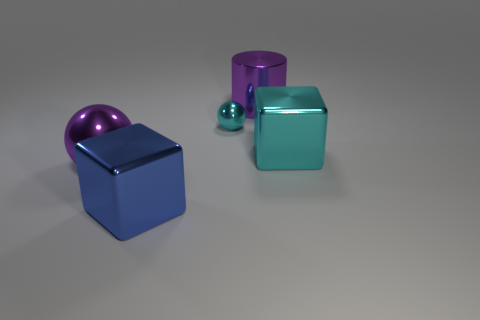
\includegraphics[width=0.5\linewidth]{figures/CLEVR_dale-5.png}
    \caption{The target object in this scene is the \emph{small turquoise sphere}. Using the incremental GRE-algorithm, the target object can be uniquely referred to as \emph{turquoise sphere}}
    \label{fig:incremental-algorithm}
\end{figure}

Given for example the scene in Figure \ref{fig:incremental-algorithm}.
Objects in this scene have three attributes that we consider in the following order of salience: a shape, a color and a size.
This order defines, which attributes can be left out, while still identifying the object uniquely.
The target object in the given scene is the \emph{small turquoise sphere}.
In the first step, the attribute with the highest salience, the shape, is selected from the target object.
This produces the referring expression \emph{sphere}.
In the next step, it is checked if there are also distractors, described by this referring expression.
In our case, both cubes and the cylinder are already disambiguated, but the purple sphere can still be described by the produced referring expression.
Therefore, the algorithm also adds the next lower salient attribute, the color to the referring expression, which produces the \emph{turquoise sphere}.
With this, also the last remaining distractor is as well disambiguated, and the referring expression describes the target object uniquely.
The size, the least salient property is therefore not necessary in the referring expression.
This algorithm will be utilized in this thesis and will be referred to as \emph{the incremental GRE-algorithm}.

Additional to generating an efficient disambiguating referring expressions, a challenge also lies in processing the visual input.
This especially applies to spatial and geometric positions and relations of objects in a scene, where models struggle to extract geometric information from visual features \citep{Kelleher2017}.
More complex scenes also involve multiple perspectives, where the models are tasked to produce referring expressions that depend on the spatial perspective of the speaker and the listener \citep{Ahrens2022,Lee2022}.
In \citep{Dobnik2021}, visual dialogue is analyzed where speakers have different views on cups that are placed on a table.
When speakers refer to a certain cup, they need to take the perspective of the listener to disambiguate the referring expression; for instance in the referring expression 'the cup on the left', \emph{left} is dependent on the speaker's and listeners' spatial position in relation to the cup.

Current research focuses hereby on generating relational referring expressions, which add more complexity to the task \citep{Ghanimifard2017,Ghanimifard2019,Ramisa2015,Liu2022a}.
Models need to first extract visual features of multiple objects from the scene.
Of these extracted objects, a meaningful landmark object needs to be found which helps to refer to the target object.
Finally, they need to find proper relations between them to describe the target object.
Relations can be mostly based on the geometric and spatial relation of two objects (e.g. above/below), while the function of objects play a stronger role in other relations (e.g. over/under) \citep{Coventry2005,Dobnik2013}.

% By doing this, the models ground parts of their language in another perception of the real world and get a step closer to learn the actual meaning.
% SD: They learn how to interpret expressions against some representation. Hence, a reference is a relation between a description and some entity, it’s interpretation. Without this connection referring expressions are useless as we do not know how to interpret this. Textual models might be good for general knowledge such as factual information from news and Wikipedia but as soon as we have NLP applications that interact with other domains, e.g. a ticket booking system or a situated robot involved in patient care, we need to connect language to some other representations to make language interpretable.
% DK: done

Referring generation tasks can be hard to evaluate, since often there are many possible referring expressions that are possible and uniquely identify the target object \citep{Mao2016}.
Instead, the task can be turned around: A model needs to identify an object when presented with a referring expression.
This is called \textbf{referring expressions comprehension}.
Many challenges remain similar to the REG task, since the model needs to extract disambiguating visual features from the scenes as well.
However, the goal is typically to select the best matching region of a given choice in a visual scene \citep{Qiao2020}.
\cmtDK[inline]{describe methods in paper}

Closely related to the REC task is visual question and answering (VQA).
In these tasks, a model is given a question about a visual scene.
The goal is to find an answer in the scene and generate an answer.
Central to this is to extract referring expressions from the question and ground them in the visual scene.
In \citep{Johnson2017}, a model is for example shown an image similar to Figure \ref{fig:incremental-algorithm} and asked the question 'Is there a blue cube with the same size as the purple cylinder?'.




\subsection{Language Games}
\label{sec:background:language-games}
\cmtDK[inline]{language games combine generation and understanding}
\cmtDK[inline]{describe as 'dialogue turns'}
\cmtDK[inline]{different approaches (robotics, neural models, ...)}
\cmtDK[inline]{different study interests (linguistically, non-linguistically)}
\cmtDK[inline]{continuous learning}
% \begin{itemize}
%     \item why language games?
%           \begin{itemize}
%               \item origins of language
%               \item flexibility
%               \item efficiency
%           \end{itemize}
%     \item setup of language game
%           \begin{itemize}
%               \item cooperative vs self-interested
%               \item asymetry
%               \item gumbel softmax vs reinforce
%               \item EGG
%               \item bottleneck
%           \end{itemize}
%     \item how does emerged language look?
%           \begin{itemize}
%               \item compositionality
%               \item generalization
%               \item efficiency
%               \item referring expressions
%               \item discriminative vs description
%               \item entropy minimization
%           \end{itemize}
%     \item why relating objects?
% \end{itemize}

The center of this thesis evolves around language games between deep neural models.
Hereby, multiple deep neural agents need to solve a task, by communicating with symbols, which initially are not associated with any meaning.
By using and interpreting these symbols in there communication, the agents start to give these symbols and their combinations meaning.
After this process, a new artificial language emerged, with which the agents can communicate with each other.
% SD: Give an example of a language games. Symbols are invented at random. However, the constraints of interaction control how new symbols are introduced and when existing symbols are re-used and used. Agents cannot invent unlimited number of symbols to refer to every event the6 encounter as they have limited memory and therefore they are driven by abstraction. On the other hand, the symbols must be flexible enough. The other agent must be able to resolve the symbols they hear based on the context. Hence, a successful interaction is when a describer is producing such symbols that interpreter can easily interpret within the context, here an image. This is also how a reward function is defined and loss is propagated.
% DK: TODO

Section \ref{sec:aims_languages} explains reasons why research in this field is conducted and how it may help in further research.
Section \ref{sec:setup-lg} shows in more detail how the language games are set up and how exactly agents can communicate and the language emerges.
Section \ref{sec:properties-el} discusses, how the emerged languages can be built up.
Finally, section \ref{sec:referring} discusses how the language games will be used in this thesis, to explore how agents can refer to objects in images.

\subsubsection{Aims of emerged languages}
\label{sec:aims_languages}
The setup of language games allows for very controlled rules of how agents can behave.
% SD: Rephrase, language games provide interactive constraints within which language can emerge. But what are these? In this thesis we will study some, such as agent’s memory and layer representation and the feature representation, the structure of the world and its ambiguity.
% DK: TODO


\subsubsection{Setup of language games}
\label{sec:setup-lg}
The term of 'language games' was first introduced by \citet{Wittgenstein1953}.
The author describes language games as uses of language between multiple interlocutors.
These can be any small parts of conversations, for instance between a teacher and a student teaching a new concept or between two persons, discussing a topic.
The rules in each of these situations differ and therefore the meanings and semantics of words and sentences may differ from situation to situation.
An interjection 'Water!' may be a warning, an answer to a question, a request or something else, depending on the context.
% SD: Because referring expressions are ambiguous participants rely on language games to resolve the reference in context.
% SD: Give an example of a game?
% DK: TODO
meanings are bound to the rules of the language games.

This reasoning was taken up, when trying to train artificial entities to produce a language.
One of the original games is the signaling game, proposed by \citet{Lewis1969}.
In this game, a sender needs to send a message to a receiver, based on information only available to the sender.
Based on the message, the receiver proposes an action.
Both sender and receiver are rewarded in the same way if the proposed action was correct.
Hence, both agents need to invent a language together, fit to the conditions of the game.

The entities can be set into real or simulated interactive situation, a language game, that meaning and a language can emerge \citep{Kirby2002}.
Multiple deep neural models, called agents, communicate with a set of symbols to solve a task.
Guided by the task and the rules, how agents can generate and interpret symbols, a language can emerge.
% SD: Examples of architectures from Baroni. The EGG framework.
% DK: TODO

% This reasoning was taken up, when trying to train deep neural models to produce language.
% These models need to be set into an interactive situation, a language game, that meaning and a language can emerge (\citet{Baroni2020}).
% Multiple deep neural models, called agents, communicate with a set of symbols to solve a task.
% Guided by the task and the rules, how agents can generate and interpret symbols, a language can emerge.

\subsubsection{Properties of the emerged language}
\label{sec:properties-el}


\subsubsection{Referring to objects and grounding}
\label{sec:referring}

\subsection{Artificial dataset}
\cmtDK[inline]{'world shapes language'}
\cmtDK[inline]{different types of biases -> reduce and control}